\chapter{Daemon design}

\section{Purpose}

\textit{Lxc} requires the processing user to have root privileges, so precautions need to be taken to ensure
the safety of the system. Mainly we do not want to have root privileges for more actions other than those who really
need these. As a consequence programs are passed to the \texttt{lxc\_daemon} who then performs the container creation
and execution and in the end returns the results back to an unprivileged program (e.g. a mail server).
A daemon (disk and execution monitor) is a background process which can only be accessed indirectly through pipes
or sockets.

\section{The Container}

Containers act like separate operating systems while sharing the kernel and the hardware resources with the host system.\\
\textit{Lxc} uses templates to create them. These are typically shell scripts which set up a minimal root
filesystem (see chapter \ref{rootfs}) in a directory (default \texttt{/var/lib/lxc/} if not specified otherwise).
The rootfs contains all files needed for the separate execution of a \textit{linux} operating system except for the kernel.
Additionally a configuration file is created which \textit{lxc} reads on container startup.\\
A container can be accessed through a command line interface or via the API.
The \texttt{lxc\_daemon} uses \textit{Debian} containers as \textit{Debian Linux}\cite{debian} is quite common and one of
the oldest and most sophisticated \textit{linux} distributions.

\section{Communication}

Any program who wants to communicate with the \texttt{lxc\_daemon} is able to do this through a unix domain socket.
Unix domain sockets are mostly handled like IP-sockets but instead of using an IP address UDS take file paths.
Also access to this socket can be limited easily through altering the file modes.
Practically speaking this allows us to only permit programs with a certain group or user id to access the socket which then again
implies that an admin has explicitly allowed this user to be able to communicate with the daemon.\\
Currently the name of the usergroup is ``lxc\_containers''.

\section{Work flow}

\begin{figure}[htb]
\begin{center}
  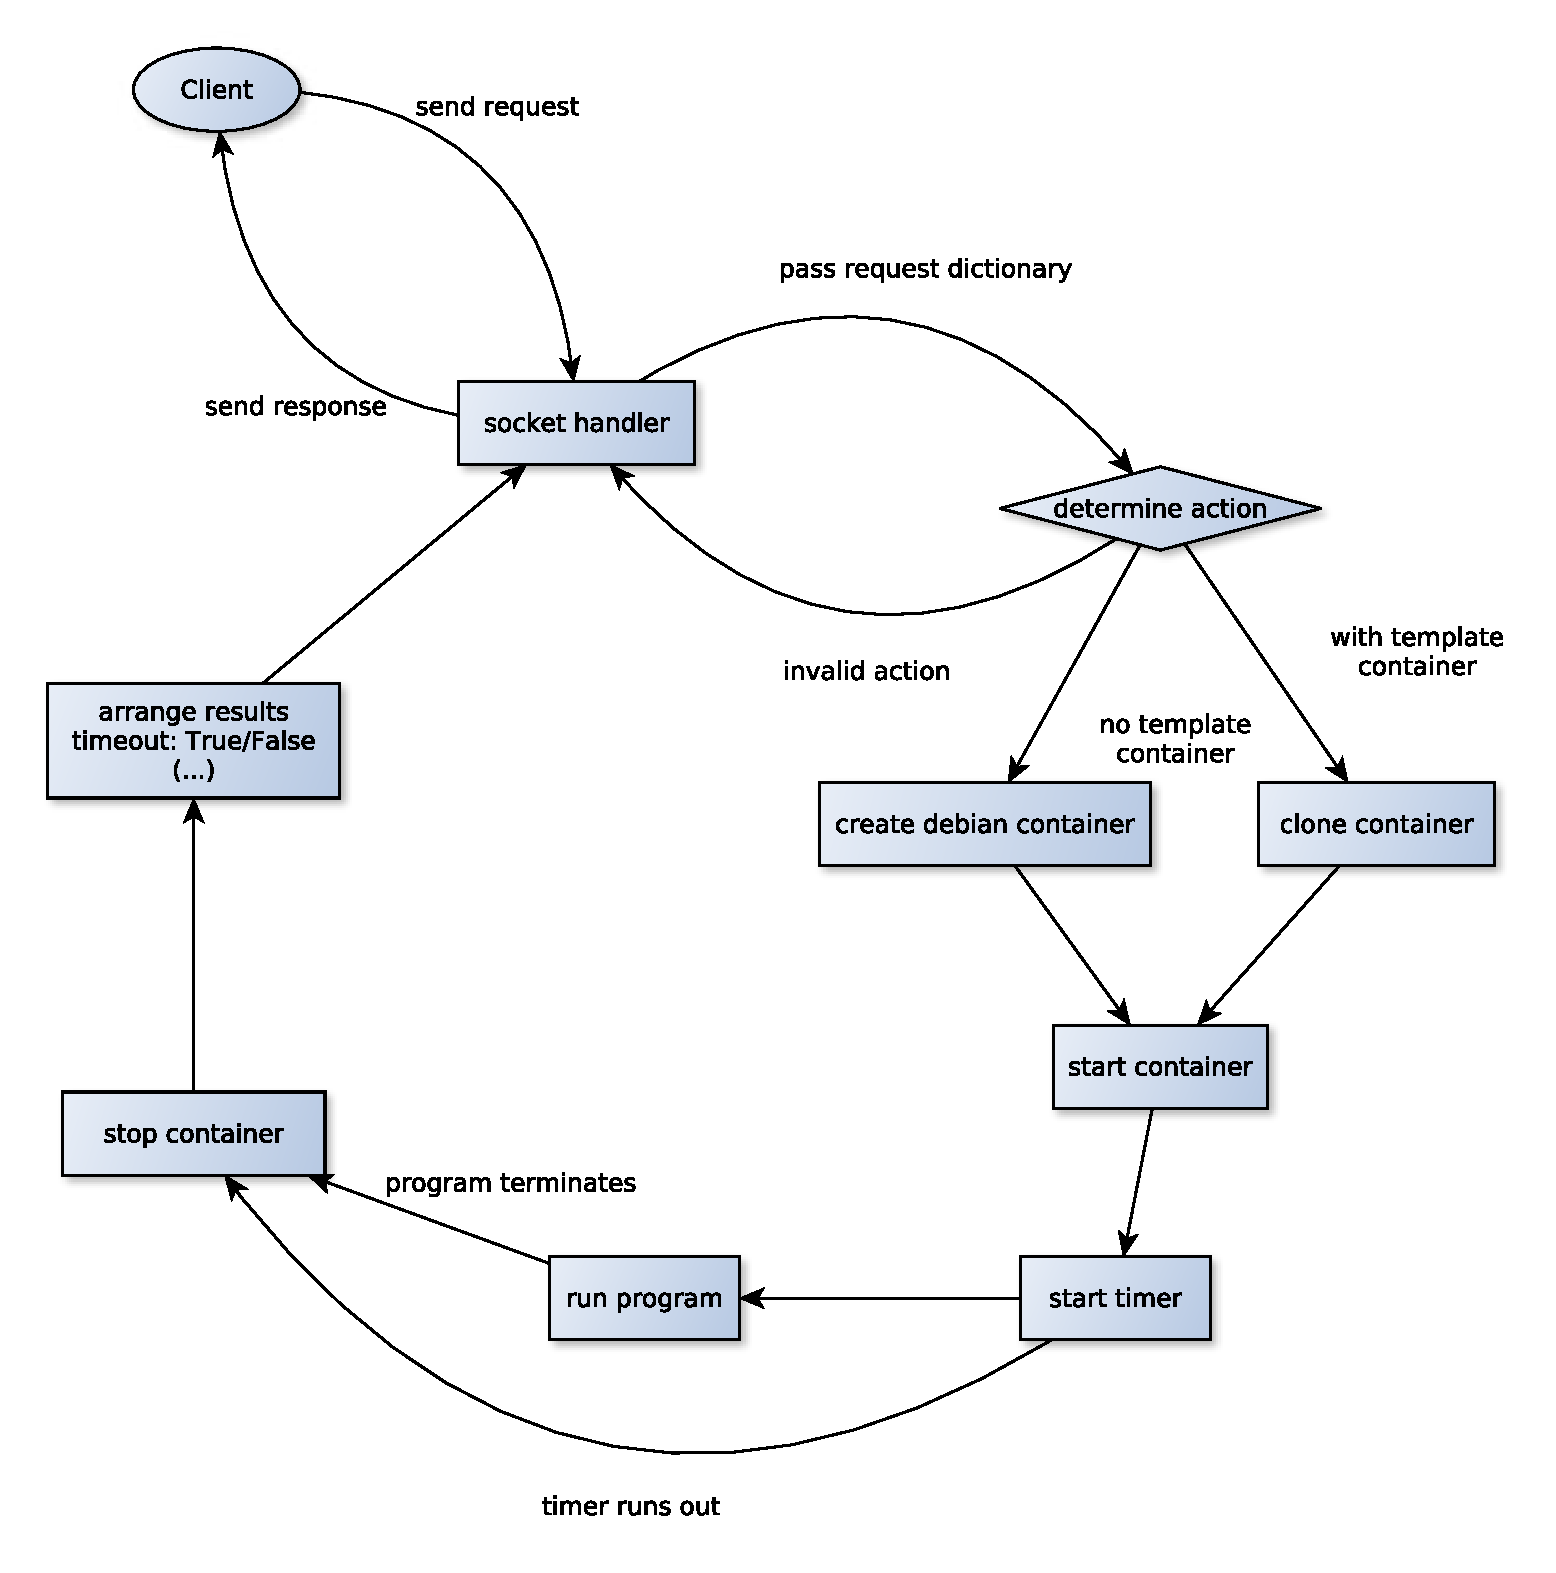
\includegraphics[width=375pt]{fig/figure_2.eps}
  \caption{work flow}
  \label{figure_2}
\end{center}
\end{figure}

When the client sends a request everything the daemon needs as information has to be provided with it.
This applies for simple keyword values as well as for files. The latter to ensure that
the corresponding unprivileged program has at least read permission for this particular file. We do
not want to execute and provide feedback on a file which may contain critical information.\\
In the next step the daemon tries to evaluate the action to be performed. If the action is unknown
a response is sent back containing information about the failure. Else the daemon checks if
a container for this session has already been created. A temporary name for the container has already
been generated when the daemon accepted the connection from the client. Assuming this is the first
request the client has asked to perform the container will most certainly not exist. In this case
the daemon consults the request again to determine whether it should create a new container or clone
from an existing one. After creation the container is started followed by the creation and starting of
a timer thread. The timeout value is either taken from the request or from a built-in constant
which serves as a fallback.
Additional files are now written into the container's rootfs if required by the current action.
Note that if the file shall be executed afterwards the file modes have to be altered accordingly as
no metadata is provided with the request.
Then the daemon attaches to the container and runs the specified command (e.g. a program written to
the rootfs one step earlier).\\
It is very important that the container is stopped, either when the program terminates or when a
timeout occurs. Otherwise \textit{lxc} will fail while trying to destroy the container causing it
to become orphaned upon closing the socket connection. Too many abandoned containers will eventually
constrain the system by using up all available resources. The daemon also makes sure that the container will be
stopped despite any internal exception.\\
When the container finally reaches the stopped state the daemon consults the request again to determine whether
it has to be destroyed or not by reading the keep alive value. This is defaulted to false so when
not specified otherwise the daemon considers the job done and closes the connection.
These steps continue from the top again if the client sends another request instead.

\section{The protocol}

The daemon takes a json object containing a python dictionary which needs to specify at least a valid action to
be performed as well as some arguments which are needed for that particular action.\\
Currently the daemon only performs the ``run\_prog'' action which requires a base64 encoded program to be run
inside the container under the keyword ``b64\_data''. Note that the base64 byte string needs to be converted to
UTF8 first as json complains when a byte string is passed.\\
In addition to that this action requires a list of parameters under the keyword ``params'' which is obligatory
because the first argument is the name of the program.\\
There are a few other non-essential options:\\
The ``keep-alive'' keyword (default: False) contains a boolean indicating whether the connection is to be closed
directly after this action or to be held open awaiting further instructions.\\
The ``timeout'' keyword (default: 60 seconds) specifies after how many seconds the container execution shall be
terminated.
Also not essential but highly recommended is the option ``use\_template\_container'' (default: None). This
requires an already existing template container from which the daemon clones a new temporary one. Not only
this is much faster than creating a container from scratch every time, but it is also an easy way to tweak
the containers for ones purposes, for example through installing additional software packages.\\
The returned json dictionary always contains a boolean variable ``success'' which if set to ``True'' should
furthermore contain any results, or if set to ``False'' some error information under the keyword ``info''.\\
The ``run\_prog'' action returns the exit value of the program and a boolean variable ``timeout'' to indicate
whether the container terminated normally or had to be shut down by the daemon.

\section{The config template}

During container
creation a generic config file is created which afterwards will be overwritten by the \texttt{lxc\_daemon} using
the template provided.
The daemon solely modifies the file paths and container name accordingly.\\
The template comprises cgroups limits and devices, a list of capabilities to drop and mountpoints.
For a detailed explanation of these see chapter \ref{features}.

\section{The timeout}

The timeout is specified in seconds and should be set to grant the executed programs a reasonable amount of time to complete
their tasks but also limit the time span where these could do harm to the system (e.g. through
writing garbage data into the rootfs) as much as possible. The daemon does not perform without
a timeout because it has to assure that the container is stopped hence it provides a fallback.\\
For the C-project in ``info 2'' the proposed value is 60 seconds. It should not take longer than that for a
project to complete its assigned tasks.

\section{Exit code evaluation}

The exit code of a program in \textit{linux} is an unsigned 8 bit integer. Retrieving this code via the python language binding
shipped with the \textit{lxc} API returns a 16 bit integer though. The 8
most significant bits are the exit code of the executed program while the 8 least significant bits indicate the exit
value of the parent process which attached to the container and tried to run the program.
If the latter fails it returns -1 which will result in the actual return value of
255 due to its unsigned nature. As a consequence any value returned by the program which is something other than 0 will be
above 255 which is why the daemon does not return the exit value directly but rather computes it as exit code modulo
255.